%"###############################################
%
% Classification RTUPB post 
%
%###############################################

En utilisant PAM sur les données post-opératoires, la courbe des silhouettes moyennes
nous indique une valeur maximale pour un nombre de classes à k = 2.

\begin{figure}[H]
\centering
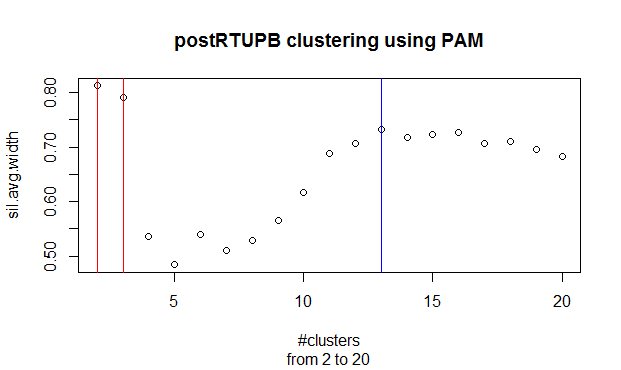
\includegraphics[width=0.90\textwidth]{../Fig/RTUPB/rtupb-elbow-post.png}
\caption{Maximisation de la silhouette moyenne }
\end{figure}

Cependant, si nous regardons le détail des classes et de leurs silhouettes pour k = 2,
nous avons une première classe incluant la quasi totalité des patients dont 2 qui ont un profil post-opératoire non relié (valeurs de silhouette négatives), et une deuxième classe ne contenant que trois patients (11, 28 et 33)
avec une valeur de silhouette à 1, indiquant des données répliquées exactement et donc une classe triviale.
Après vérification que ces patients ont des données post-opératoires identiques, mais ne sont pas pour autant
des doublons (données pré-opératoires différentes), nous poursuivons la recherche jusqu'au maximum suivant qui se trouve à k = 3.

\begin{figure}[H]
\centering
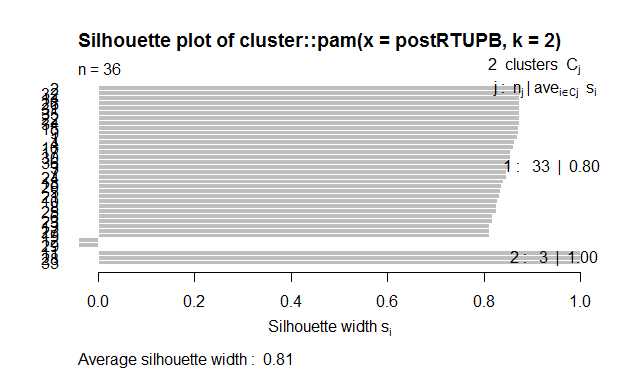
\includegraphics[width=0.75\textwidth]{../Fig/RTUPB/rtupb-sil-k2-post.png}
\caption{Silhouette / classe (k = 2) }
\end{figure}

En examinant, pour k = 3, la répartition des classes et leurs silhouettes, nous faisons le même constat que précédemment, et une nouvelle classe triviale (patients 12 et 29) est apparue pour des patients distincts
mais dont les données post-opératoires sont identiques. Nous poursuivons encore la recherche jusqu'au maximum suivant qui se trouve à k = 13.

\begin{figure}[H]
\centering
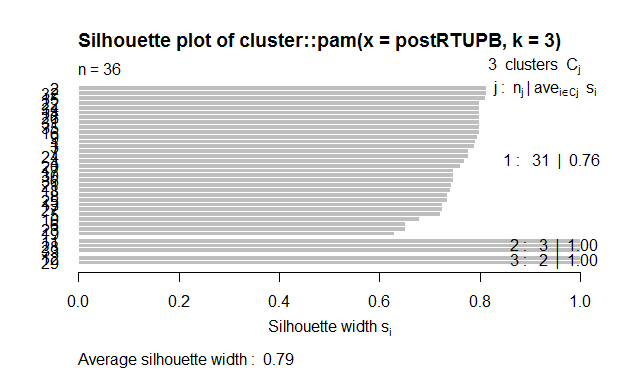
\includegraphics[width=0.75\textwidth]{../Fig/RTUPB/rtupb-sil-k3-post.png}
\caption{Silhouette / classe (k = 3)}
\end{figure}

Le partitionnement à 13 classes permet d'identifier 10 classes de profils post-opératoires bien voire très bien classés: 3 dont la silhouette vaut 1, 5 dont la silhouette est comprise entre 0.75 et 1, et 2 dont la silhouette
est aux alentours de 0.6). Ce partitionnement fait également apparaître 2 classes de profils post-opératoires pas très bien classés (silhouette < 0.5) et une classe singleton (silhouette = 0). 

\begin{figure}[H]
\centering
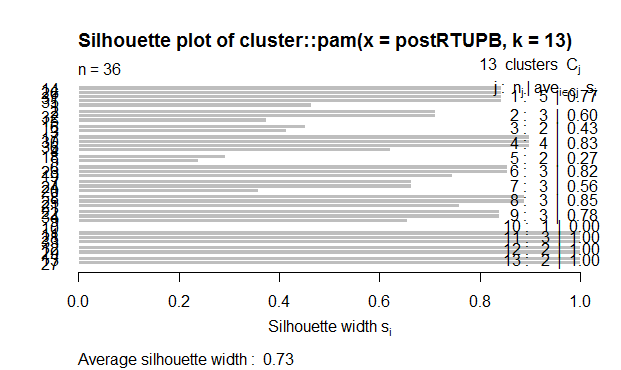
\includegraphics[width=0.75\textwidth]{../Fig/RTUPB/rtupb-sil-k13-post.png}
\caption{Silhouette / classe (k = 13)}
\end{figure}

La classification hiérarchique favoriserait plutôt un niveau de coupure de l'arbre correspondant à un partitionnement à 4 classes. Le partitionnement à 13 classes représente le niveau de coupure suivant et représenté en rouge sur la figure ci-dessous.

\begin{figure}[H]
\centering
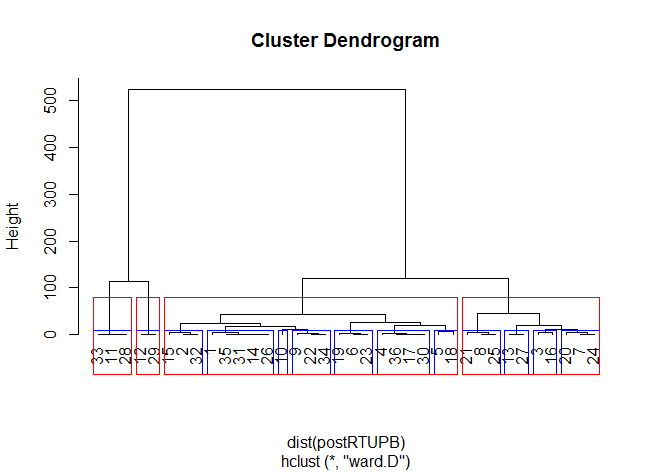
\includegraphics[width=0.75\textwidth]{../Fig/RTUPB/rtupb-cah-k13-post.png}
\caption{Silhouette / classe (k = 13)}
\end{figure}

Comme nous le verrons en étudiant les profils de guérison, les partitionnements à respectivement 4 ou 13 classes sont cohérents entre eux. 

%
%##########################
%# CONCLUSION
%##########################